\documentclass[12pt, a4paper]{article}
\title{Overhead Crane 2-Axis Positioning}
\author{Ryan Lederhose}
\date{May 2023}
\usepackage{graphicx, adjustbox, lipsum, float, amsmath}
\graphicspath{{./images/}}

\begin{document}
\maketitle

\newpage

\begin{abstract}
ABSTRACT
\end{abstract}

\newpage

\tableofcontents

\newpage

%%%%%%%%%%%%%%%%%%%%%%%%%%%%%%%%%%%%%%%%%%%%%%%%%%%%%%%%%%%%%%%
%%                       INTRODUCTION                        %%
%%%%%%%%%%%%%%%%%%%%%%%%%%%%%%%%%%%%%%%%%%%%%%%%%%%%%%%%%%%%%%%
\section{Introduction}
The main aim of this project is to develop a functioning prototype for Bluescope Steel Acacia Ridge to assist in auditing the travel path and lift rating of overhead cranes. 
\subsection{Motivation}
It has long been identified that human error is the leading cause of incidents in the workplace and thus Bluescope has always prioritised the health and safety of its workers. Bluescope Acacia Ridge has six overhead cranes on-site which are used by the operators to move steel coils. The overhead cranes pose a safety risk to the operators, and with the correct data, it is possible to introduce safety measures that would lower the risk to operators in the field.
\subsection{Background}
Bluescope have provided a real-time location system (RTLS) solution from Pozyx. The software development kit (SDK) uses anchors (stationary transceivers) to aid in positioning one or more tags (non-stationary transceivers) in a given area. Bluescope believe that with the provided software development kit, the real-time position of the overhead cranes can be captured at regular intervals. Furthermore, by integrating the real-time position with the hook weight, Bluescope can develop a heat map of the warehouse floor, indicating heavy traffic areas so appropriate measures can be introduced to reduce risks.
\subsubsection{Pozyx RTLS Solution}
The provided software development kit uses stationary transceivers, hereafter referred to as anchors, to accurately position the location of non-stationary transceivers, hereafter referred to as tags. The SDK uses a positioning protocol known as Two-way-ranging (TWR).

In TWR, the distance from a tag to an anchor is measured by sending a data packet between the two transceivers. By measuring how long it took for the packet to return, the tag can estimate the distance to the anchor. If the tag has ranged with at least three anchors, it can compute its position in the given area through trilateration [2]. This consequently means the coordinates of all anchors must be known prior to positioning.

In this particular solution, one master tag instructs one or more remote tags to position themselves through the anchors. This master tag is connected to a computer or microcontroller which in turn retrieves the position from all the remote tags. Alternatively, it is possible to position the master tag itself, however, this does not scale well to large areas [2].

The anchors and tags communicate between each other through ultra-wideband (UWB) technology. UWB is a shortrange, very high frequency, wireless communication protocol that uses radio waves [1]. Consequently, UWB has problems transmitting through walls and is heavily interfered by surrounding metal. It ultimately works best if there is a clear line-of-sight between transmitter and receiver. 

UWB provides a low spectral density and wide bandwidth solution to wireless communication as such:
\begin{figure}[h]
    \centering
    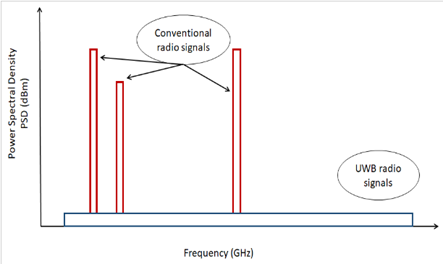
\includegraphics[width=0.85\textwidth]{UWB vs PSD.png}
    \caption{Ultra-wideband Frequency versus Power Spectral Density [1]}
    \label{fig:uwb_psd}
\end{figure}
\newline
UWB features are highlighted below: [1]
\begin{itemize}
    \item Wide bandwidth provides immunity against the channel effect, especially in a dense environment
    \item UWB systems can co-exist with existing narrowband systems
    \item UWB enables high data rates over short distances
    \item Low spectral density ensures low probability of signal detection and consequently increases security of connection
\end{itemize}
The Pozyx RTLS solution has four anchors and six tags, with one of these tags serving as a master tag. The master tag talks to its host device either through a serial port or an I2C connection. Pozyx claim the solution is 10cm accurate with a 60Hz update rate locally, or up to 45Hz remotely. The range of the transceivers is 30m, with Pozyx suggesting four anchors can cover a space of $400 – 800m^2$. They additionally advise a few rules be followed when placing the anchors:
\begin{enumerate}
    \item Place the anchors high and in line-of-sight of the user
    \item Spread the anchors around the user, never place them in a straight line
    \item Place the anchors vertically with the antenna at the top
    \item Keep the anchors away from the metal - it is advised to keep 20cm clear from the antenna to the metal
\end{enumerate}

\subsubsection{IEEE 802.15.4}
IEEE 802.15 is a working group of the IEEE 802 standards committee which specifies wireless personal area network (WPAN) standards. More specifically, IEEE 802.15.4 specifies the physical layer (PHY) and media access control (MAC) layer of the Open Systems Interconnection (OSI) model of network operation.

The physical layer defines the power modulation, frequency and other wireless conditions of the link whereas the MAC layer defines the format of the data handling [5]. The standard provides a basis to which other features could be added through the upper layers. Zigbee is the most common enhancement of the 802.15.4 standard [5]. 
\begin{figure}[h]
    \centering
    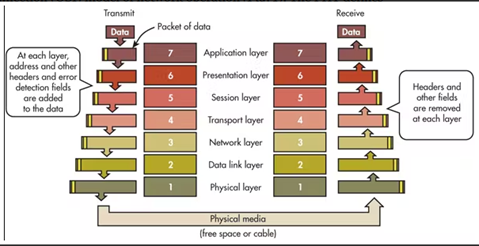
\includegraphics[width=0.75\textwidth]{osi model.png}
    \caption{Open Systems Interconnection Model of Network Operation [5]}
    \label{fig:osi_model}
\end{figure}
\newline
Zigbee is a mesh network protocol, which means that devices can communicate directly with each other, or they can relay messages through other devices in the network. This allows Zigbee devices to create a self-healing network that can continue to function even if some devices are out of range or out of power. There are three classes of Zigbee devices:
\begin{itemize}
    \item Zigbee Coordinator: The coordinator forms the root of the network tree. There is always precisely one coordinator in each network since it is the device that started the network originally
    \item Zigbee Router: Routers can both run an application function and pass data on to other devices
    \item Zigbee End Device: Contains just enough functionality to talk to a router or coordinator. These devices cannot relay data and simply run an application function, fetching data and transmitting it into the mesh network
\end{itemize}
One of the key features of Zigbee is its low power consumption. Zigbee devices can run for several years on a single battery, 
making it well suited for use in remote or hard-to-reach locations. Additionally, Zigbee devices can operate in both sleep and 
active modes, which allows them to conserve power by only transmitting data when necessary.

Zigbee also has a high level of security built-in, providing data encryption and device authentication, 
making it a secure option for industrial and commercial applications.

\subsubsection{Electronic Filters}
Electronic filters will allow certain signals to pass through while attenuating others based on the physical architecture of the circuit. 
There are four major electronic filter types – low pass, high pass, band pass and band stop. There response curves are shown below:
\begin{figure}[h]
    \centering
    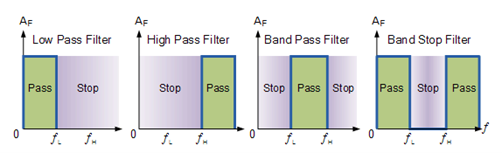
\includegraphics[width=0.75\textwidth]{filters.png}
    \caption{Ideal Filter Response Curves [3]}
    \label{fig:filter_curves}
\end{figure}
\newline
When converting an analog signal to a digital output via an ADC, it is important to filter the analog input with a 
low pass filter. A low pass filter will allow low frequencies to pass through but will attenuate the high frequencies [3] 
and hence by using a low pass filter on an analog input, the signal becomes less noisy, with the high frequency components 
being attenuated by the filter. This reduces the risk of aliasing, the phenomenon where new frequencies appear on a sampled signal after reconstruction.  

A low pass filter can be constructed through a simple RC circuit:
\begin{figure}[h]
    \centering
    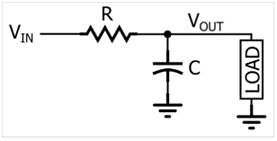
\includegraphics[width=0.6\textwidth]{rc cct.png}
    \caption{RC Low-Pass Filter [4]}
    \label{fig:rc_cct}
\end{figure}
\newline
At low frequencies, the capacitor acts as an open circuit, allowing the signal to pass to the load; however, 
at higher frequencies the capacitor will act as a short circuit, essentially grounding the signal. The frequency 
in which the circuit will begin attenuating the signal is defined as the cut-off frequency.
\subsection{Objectives}
The goal of this project is to develop a working prototype of a system capable of capturing the instantaneous 
2-axis position of an overhead crane and its hook weight at periodic and synchronised units of time. The system must 
use the provided RTLS solution to synchronise position and weight to store in an external database with a given timestamp. 
The synchronised data must be repeatable for long term use. The system must be adaptable for use across all cranes on-site. 
\subsection{Scope}
It is in scope of the project to:
\begin{itemize}
    \item Determine optimal positions and number of tags and anchors for application
    \item Accurately retrieve position of crane hook in 2 dimensions using supplied anchors, tags and SDK
    \item Accurately retrieve hook weight at periodic units of time
    \item Synchronise data from RTLS system and weight sensor
    \item Develop custom software to capture hook weight and instantaneous position of the overhead crane and store in an external database at regular intervals
    \item Benchmark accuracy of system
    \item Testing of various failover scenarios and recovery (e.g. loss of database connection, loss of anchor connection)
    \item Develop a software test plan to test the prototype for all outcomes and scenarios using Crane 3 as a test site
    \item Develop a plan for a site-wide roll out of the prototype considering the different challenges for each crane
\end{itemize}
\subsection{Assumptions}
To complete this project, several assumptions had to be made:
\begin{itemize}
    \item Load gauge attached to the cranes provides a clean 0-10V analog signal
    \item Bluescope will provide a method of wiring the load gauge signal
    \item Bluescope will provide correct power supplies
    \item Bluescope will cover cost of production and labour
    \item Bluescope will provide a method of mounting tags, anchors and necessary equipment
    \item A network connection will be made available
\end{itemize}

\newpage

%%%%%%%%%%%%%%%%%%%%%%%%%%%%%%%%%%%%%%%%%%%%%%%%%%%%%%%%%%%%%%%
%%                       POSITIONING                         %%
%%%%%%%%%%%%%%%%%%%%%%%%%%%%%%%%%%%%%%%%%%%%%%%%%%%%%%%%%%%%%%%
\section{Real-Time Positioning}
The scope and objective of the project requires the positioning system to meet the following requirements:
\begin{itemize}
    \item Metre-by-metre accuracy
    \item Update rate great enough to capture metre-by-metre travel path of crane
    \item Error checking and boundary condition handling
\end{itemize}
\subsection{Crane 3 Layout}
For testing and design purposes crane 3 was used. The crane covers an area of 21.86m x 84m ($1836.24m^2$). The area encompasses 
Bay 3, Bay 7 and rows of coil storage separating the two bays. Moreover, it is lined on the east and west sides by metal pillars, 
each separated by 7.6m. These pillars stretch up to the roof of the warehouse. (APPENDIX FOR SCHEMATIC)

The crane is typically used by dispatch, to move coils from Bay 3 and the surrounding rows to Bay 7, where they will get 
loaded onto trucks by forklifts. In the case of wet weather, the trucks may be loaded inside the warehouse by the crane itself. 
The crane is also commonly used for repacking coils, where coils will be loaded onto the down-ender for turnovers by the crane.

The technical specifications for crane 3 are found in detail in Appendix 2, but are also summarised below for convenience:
\begin{center}
    \begin{table}[h]
        \begin{adjustbox}{width=1.2\textwidth, center=\textwidth}
            \small
            \begin{tabular}{||c c c c c c c||}
                \hline
                Span & Height of Lift & Traverse Speed & Hoisting Speed & Long Travel Speed & Weight of Hoist & Power Supply \\
                \hline
                21.522m & 9m & 0.667m/s & 0.0533m/s & 1.0833m/s & 2.5T & 415V / 50Hz \\
                \hline
            \end{tabular}
        \end{adjustbox}
        \caption{Technical Specifications of Crane 3}
        \label{tab:crane_3_specs}
    \end{table}
\end{center}
\subsection{Initial Design}
For an initial design a NucleoL432KC development board was used. This board uses a STM32L432KCU6 microcontroller. 
STM32 microcontrollers are widely supported by STMicroelectronics and the community. These microchips generally have a wide range of 
peripherals, including I2C, USART and ADC, making them a great option to develop firmware on. The connections between the development board and 
master tag are as described in Figure \ref{fig:nuc_tag_cct}.
\begin{figure}[h]
    \centering
    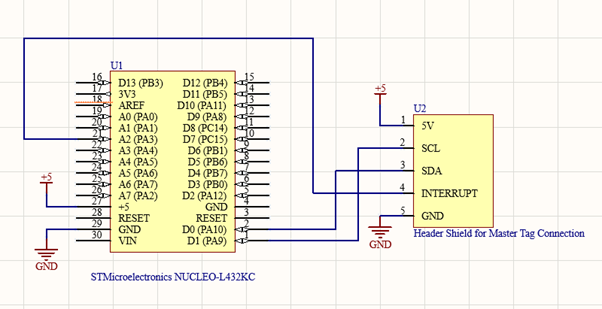
\includegraphics[width=0.9\textwidth]{nucleo to tag.png}
    \caption{NucleoL432KC Board to Master Tag Schematic}
    \label{fig:nuc_tag_cct}
\end{figure}
\subsubsection{Positioning Accuracy}
Pozyx offers a range of customisation options for the positioning system. The \textit{POZYX\_POS\_FILTER}
register offers the programmer options for configuring positioning filters by the device. The register offers four filter options: none, FIR, moving 
average and moving median. Additionally, the device allows the user to configure the strength of the filter; a value between 0 and 15 indicating 
the number of samples the position will be delayed by. Moreover, the \textit{POZYX\_POS\_ALG}
register will allow the programmer to configure the dimension and algorithm used by the position function. 
Dimensions available are 2D, 2.5D and 3D; however, the scope only requires and x-y position hence, 2D is the logical option. 
Algorithms available are UWB and Tracking; however, tracking is only available for 3D positioning hence, UWB is the only option. 

For an initial test four anchors were used, each attached to a seperate pillar 2.5m above the ground in the arrangment described by Figure \ref{fig:setup1}.
\begin{figure}[h]
    \centering
    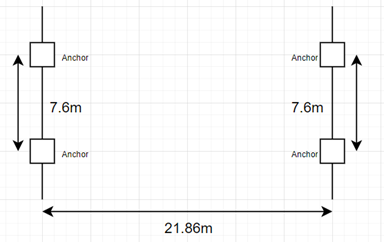
\includegraphics[width=0.8\textwidth]{setup1.png}
    \caption{21.86m x 7.6m Anchor Setup}
    \label{fig:setup1}
\end{figure}
In this arrangment, the anchors cover an area of $166.136m^2$, which falls in the recommended range for anchor placement by Pozyx. 
It was understood that the metal pillars would interfere with the anchor-tag transmission, however, at such short range, 
the effects were considered negligible. The \textit{POZYX\_POS\_FILTER} register was customised such that a moving 
average filter set to a strength of 10 was configured for positioning to allow for a smooth trajectory and a high sample rate. It should be 
noted that during this test the update rate was not considered to be a variable worth testing.

For this test, the master tag was positioned in a known location and the position calculated by the tag is compared to the actual value. The results are described in Table \ref{tab:res1}.
\begin{center}
    \begin{table}[h]
        \begin{adjustbox}{width=1\textwidth, center=\textwidth}
            \small
            \begin{tabular}{||c c c||}
                \hline
                Actual Position (mm, mm) & Calculated Position (mm, mm) & Percent Error \\
                \hline
                (1000, 0) & (990, 70) & 1\% \\
                \hline
                (0, 1000) & (10, 1005) & 0.5\% \\
                \hline
                (10900, 3800) & (10915, 3790) & 0.26\% \\
                \hline
                (21000, 7000) & (21048, 6950) & 0.22\% \\
                \hline
            \end{tabular}
        \end{adjustbox}
        \caption{21.86m x 7.6m Accuracy Test}
        \label{tab:res1}
    \end{table}
\end{center}
The results show that within the designated test area, the master tag was able to position itself accurately on the ground floor with an error
$\leq$1\%. As the results were promising, the test area was widened to a 15.2m x 21.86m area as such:
\begin{figure}[H]
    \centering
    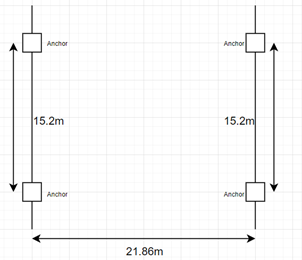
\includegraphics[width=0.7\textwidth]{setup2.png}
    \caption{21.86m x 15.2m Anchor Setup}
\end{figure}
For this test, the master tag was no longer going to be performing position, but rather a remote tag, simulating a more realistic condition closer to that
of the final product. The results are shown below:
\begin{center}
    \begin{table}[h]
        \begin{adjustbox}{width=1\textwidth, center=\textwidth}
            \small
            \begin{tabular}{||c c c||}
                \hline
                Actual Position (mm, mm) & Calculated Position (mm, mm) & Percent Error \\
                \hline
                (1000, 0) & (1023, 26) & 2.3\% \\
                \hline
                (0, 1000) & (20, 1052) & 5\% \\
                \hline
                (7600, 10930) & (7892, 11334) & 3.4\% \\
                \hline
                (15000, 21000) & (15447, 21069) & 2.9\% \\
                \hline
            \end{tabular}
        \end{adjustbox}
        \caption{21.86m x 7.6m Accuracy Test}
        \label{tab:res2}
    \end{table}
\end{center}
Expanding the test area evidently increased the percentage error in the results. The scope of the project requires a metre-by-metre map
of the travel path of the crane. Hence, variances in positions of up to 0.5m can be ignored and ultimately not affect the outcome
meaningfully. Thus, the increase in percentage error for this test can be considered insignificant.

An observation made during this test is that the connection between the remote tag and master tag would experience interference
intermittently, with it being prevalent when the remote tag was taken into the rows of coils north of Bay 3. Unfortunately, interference,
is an inherit issue that was encountered, especiialy in the test area. The area has a number of steel coils always present. The metal interrupts
the UWB signal through blocking line-of-sight and diminishing the strength of the signal. The interference issues encountered demonstrate
how essential line-of-sight is in UWB transmission and how it must be prioritised when designing the final layout and prototype 
of the system.


\newpage

%%%%%%%%%%%%%%%%%%%%%%%%%%%%%%%%%%%%%%%%%%%%%%%%%%%%%%%%%%%%%%%
%%                       HOOK WEIGHT                         %%
%%%%%%%%%%%%%%%%%%%%%%%%%%%%%%%%%%%%%%%%%%%%%%%%%%%%%%%%%%%%%%%
\section{Hook Weight}
The load gauge attached to Crane 3 outputs a 0-10V analog signal which varies as the weight on the hook changes.
Using an analog-to-digital converter (ADC), the signal can be processed and discretised, such that the hook weight can be calculated.

The scope of the project requires the hook weight be calculated at periodic intervals of time with an accuracy of 0.1T. 
\subsection{Analog-to-Digital Converter Circuit Design}
The logical choice for an ADC is on-board most STM32 microntrollers. This eliminates the need for another IC, as well as facilitating
easy configuration within the STM32CubeIDE, including configuration for a 12-bit reading. The most common input range for a single-ended ADC 
is 0-3.3V. Since the input from the load gauge is 0-10V, the signal must be transformed. 
\subsubsection{Voltage Divider}
To transform the voltage, a simple voltage divider was used:
\begin{figure}[h]
    \centering
    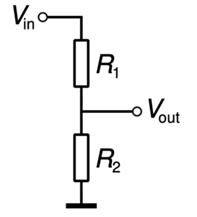
\includegraphics[width=0.3\textwidth]{voltage divider.png}
    \caption{Voltage Divider Circuit}
    \label{fig:v_divider}
\end{figure}

\[V_{out}= V_{in}*\frac{R_2}{R_1+R_2}\]
Assuming $R_2=15k\Omega$ \& considering the peak voltages (i.e. $V_{in}=10V,  V_{out}=3.3V$), $R_1$ is then calculated:

\[3.3=10*\frac{15*10^3}{R_1+15*10^3}\]
\[R_1=30.5k\Omega\]
It should be noted that $R_2$ was assumed to be $15k\Omega$ such that it did not draw significant current from the source. 
With the voltage transformed to a 0-3.3V signal, high frequency components in the signal creating noise needed to be considered. 

\subsubsection{Frequency Analysis}
A low pass filter was constructed with an RC circuit, with the voltage divider forming the resistor component as such:
\begin{figure}[h]
    \centering
    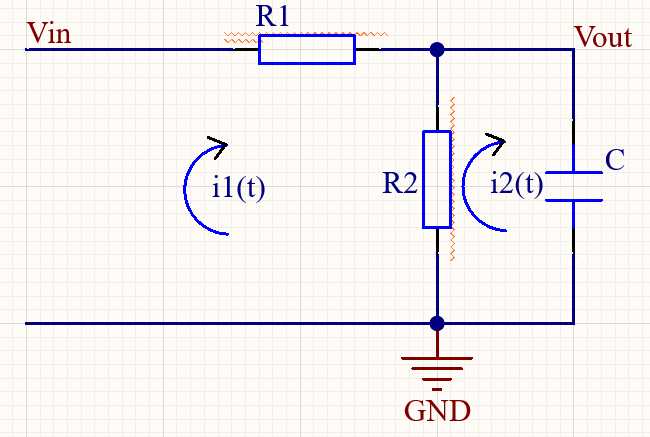
\includegraphics[width=0.5\textwidth]{kvl.png}
    \caption{RC circuit with Voltage Divider}
    \label{fig:rc_w_vdivider}
\end{figure}

To avoid aliasing, the cut off frequency of the low pass filter should be no more than half the sample rate of the ADC. 
Assuming a sample rate of 2Hz, matching that of the positioning, 
the cut off frequency of the low pass filter will be 1Hz; Thus, the capacitance of the circuit is:

\[f_c=\frac{1}{2{\pi}RC}\]
\[C=\frac{1}{2{\pi}15k//30.5k}  {\approx}  20{\mu}F \]
To calculate the frequency response of this circuit, the circuit can be taken to the s-domain as such:


Taking KVL for Figure \ref{fig:rc_w_vdivider} the following equations are yielded:
\[V_{in}=R_1i_1(t)+R_2(i_1(t)-i_2(t))\]
\[0=R_2(i_2(t)-i_1(t))+\frac{1}{C}\int i_2(t) \,dt\]
\[V_{out}=\frac{1}{C}\int i_2(t) \,dt\]
\indent The Laplace transform of the simulataneous equations gives:
\[V_{in}(s)=R_1I_1(s)+R_2(I_1(s)-I_2(s))\]
\[0=R_2(I_2(s)-I_1(s))+\frac{1}{Cs}I_2(s)\]
\[V_{out}(s)=\frac{1}{Cs}I_2(s)\]
\indent Writing these equations in matrix form,
$$
    \begin{pmatrix}
        V_{in}(s) \\
        0 
    \end{pmatrix} =
    \begin{pmatrix}
        R_1+R_2 & -R_2 \\
        -R_2 & \frac{1}{Cs}+R_2
    \end{pmatrix}
    *
    \begin{pmatrix}
        I_1(s) \\
        I_2(s)
    \end{pmatrix}
$$
\indent Rearranging for $I_1(s)$ and $I_2(s)$,
$$
    \begin{pmatrix}
        I_1(s) \\
        I_2(s)
    \end{pmatrix} =
    \frac{1}{\Delta} *
    \begin{pmatrix}
        \frac{1}{Cs}+R_2 & R_2 \\
        R_2 & R_1+R_2
    \end{pmatrix}
    *
    \begin{pmatrix}
        V_{in}(s) \\
        0 
    \end{pmatrix}
$$
\indent Where $\Delta$ is,
$$
    \Delta = (R_1+R_2)(\frac{1}{Cs}+R_2)-R_2^2
$$
\indent Solving for $I_2(s)$ gives,
\[I_2(s)=\frac{1}{(R_1+R_2)(\frac{1}{Cs}+R_2)-R_2^2}*R_2*V_{in}(s)\]                                                                                                                                                                                                                                                                                                                                                                                                                                                                                      
\[I_2(s)=\frac{R_2Cs}{R_1+R_2+R_1R_2Cs}*V_{in}(s)\]
\indent Substituting in the values for $R_1=30.5k\Omega$, $R_2=15k\Omega$, $C=20{\mu}F$ and $I_2(s)=V_{out}(s)Cs$,
\[V_{out}(s)=\frac{15*10^3}{15*10^3*30.5*10^3*20*10^{-6}s+(30.5+15)*10^3}*V_{in}(s)\]
\[V_{out}(s)=\frac{15}{9.15s+45.5}*V_{in}(s)\]
\[V_{out}(s)=\frac{1}{0.61s+3.033}*V_{in}(s)\]
\indent Hence, the transfer function of the system is,
\[\frac{V_{out}(s)}{V_{in}(s)}=\frac{1}{0.61s+3.033}\]
The corresponding bode plot of the transfer function is:
\begin{figure}[H]
    \centering
    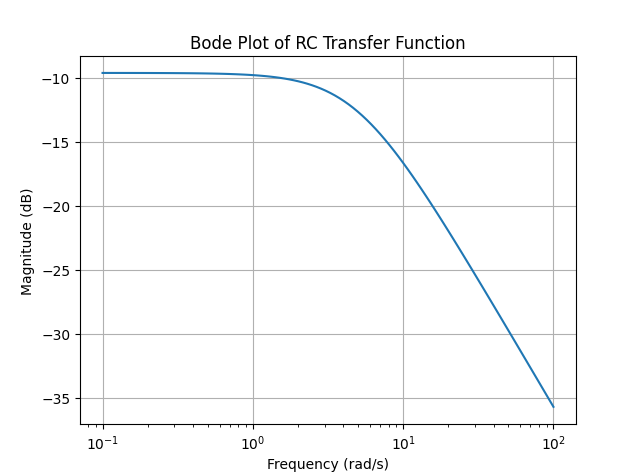
\includegraphics[width=0.75\textwidth]{bodeplot}
    \caption{Bode Plot of Transfer Function}
    \label{fig:bode_plot}
\end{figure}
\noindent Figure \ref{fig:bode_plot} shows that at steady state the system experiences small attenuation, $\approx-9dB$,
hence it can be expected that for a max input of 10V, the system will not transform the signal to a 3.3V peak, but rather
bound the signal to near 3.2V due to impedance provided by the capacitor.
The difference of $\approx 0.1V$ is ultimately negligible when considering the scope of the project.

The transfer function indicates the system has one real pole at $s=-4.972$. This indicates that the system is:
\begin{enumerate}
    \item Stable - Left-hand plane poles are stable, bounds the output with decaying exponential
    \item Non-periodic - Complex conjugate poles result in oscillatory behaviour in the time-domain, real poles do not.
\end{enumerate}
\subsubsection{Time-Response Analysis}
\indent Assuming $V_{in}(t)=Vu(t) \rightarrow V_{in}(s)=\frac{V}{s}$, solving for the time-response by performing partial fraction expansion gives,
\[V_{out}(s)=\frac{1}{s(0.61s+3.033)}*V\]
\[\frac{1}{s(0.61s+3.033)}=\frac{A}{s}+\frac{B}{0.61s+3.033}\]
\indent \indent Letting $s=0$ gives,
\[A=0.32\]
\indent \indent Letting $s=-4.97$ gives,
\[B=-0.2\]
\indent \indent Therefore,
\[V_{out}(s)=V\left(\frac{0.32}{s}+\frac{-0.2}{0.61s+3.033}\right)\]
\indent \indent Taking the Inverse Laplace Transform,
\[V_{out}(t)=0.32V\left(1-0.625e^{-4.07t}\right)u(t)\]
Graphing this time response to a 10V input ($V=10V$) yields the following result,
\begin{figure}[H]
    \centering
    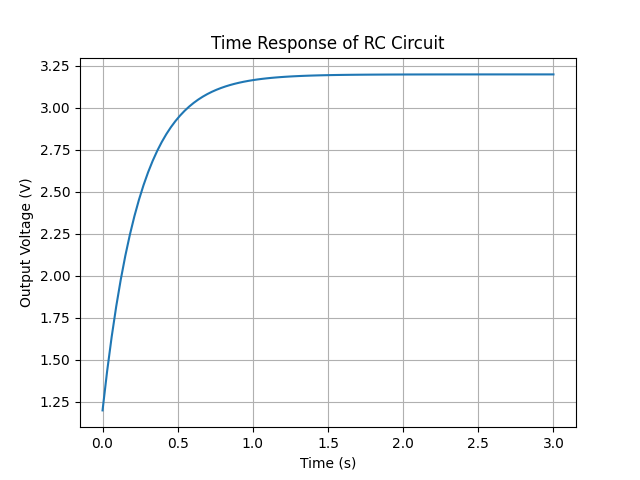
\includegraphics[width=0.75\textwidth]{graph10.png}
    \caption{RC Circuit Time Response to 10V Input}
    \label{fig:time_response}
\end{figure}
As seen in Figure \ref{fig:time_response}, the output voltage is bounded to $\approx3.24V$, with transient response characteristics of:
\begin{itemize}
    \item Time Constant = 0.2 seconds
    \item Settling Time = 0.8 seconds
    \item Rise Time = 0.44 seconds
\end{itemize}
The settling and rise time of the transient response is indicative of smooth and fast feedback to a step input, meeting the scope of the project.
\subsubsection{Buffer Amplifier}

The single-ended ADC input on STM32 microcontrollers typically have high input impendance of around $40k\Omega$. This in turn affects the analog
input voltage, decreasing its magnitude. To counteract this issue, a buffer amp follows the RC circuit essentially decoupling the circuit from the ADC input. The result
leads to the following schematic:
\begin{figure}[H]
    \centering
    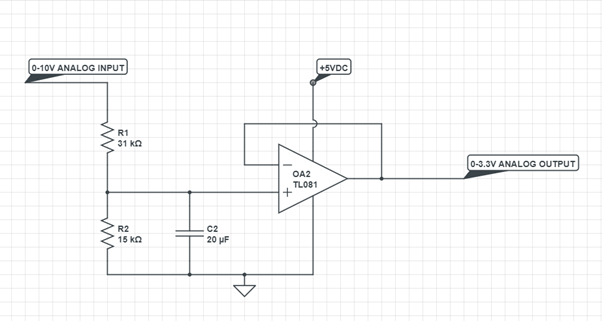
\includegraphics[width=0.9\textwidth]{adc_cct.png}
    \caption{ADC Circuit Schematic}
    \label{fig:adc_schem}
\end{figure}
\subsection{ADC Circuit Test}
The ADC circuit in Figure \ref{fig:adc_schem} was tested using the Portacal 1000 to supply a 0-10V analog signal. The output from the buffer
amplifier was wired into a single-ended ADC input on the NucleoL432KC board. The analog signal was converted by the STM32,
and the digital result was pushed out to a serial port. The results from the test are as followed:
\begin{center}
    \begin{table}[h]
        \begin{adjustbox}{width=0.7\textwidth, center=\textwidth}
            \small
            \begin{tabular}{||c c c c c c||}
                \hline
                Analog Input (V) & 2 & 4 & 6 & 8 & 10 \\
                \hline
                Raw ADC Strain & 632 & 1455 & 2265 & 3082 & 3864 \\
                \hline
            \end{tabular}
        \end{adjustbox}
        \caption{ADC Circuit Test Result}
        \label{tab:res3}
    \end{table}
\end{center}
\subsubsection{Regression Analysis}
Plotting the data in Table \ref{tab:res3} and performing a regression analysis using the sklearn.linear\_regression.LinearRegression library yields the following
result:
\begin{figure}[H]
    \centering
    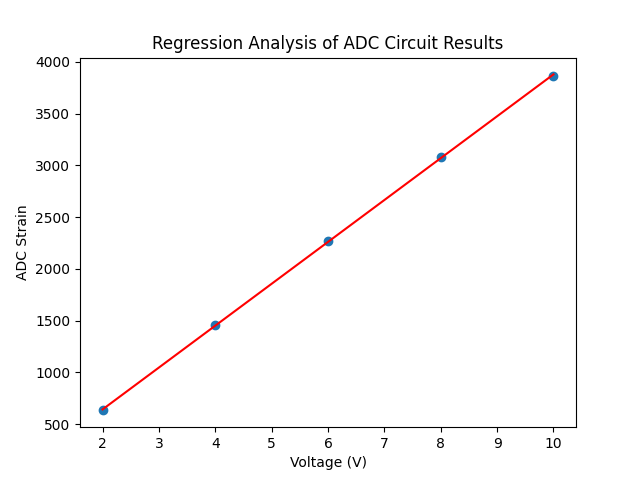
\includegraphics[width=0.75\textwidth]{adc_graph.png}
    \caption{Linear Regression Analysis of Table \ref{tab:res3}}
    \label{fig:regr_test}
\end{figure}
\begin{center}
    Predicted Function: $y=405.55x-167.7$; 
    Sum Squared Errors: $SSE=505$
\end{center}
The results of the regression analysis indicate the relationship between the ADC strain and voltage is linearly proportional, with the linear regression
model able to predict ADC strains with little error. The accuracy of the model indicates that a similar process can be used to calculate the hook weight.



\newpage

%%%%%%%%%%%%%%%%%%%%%%%%%%%%%%%%%%%%%%%%%%%%%%%%%%%%%%%%%%%%%%%
%%                       DATABASE STORAGE                    %%
%%%%%%%%%%%%%%%%%%%%%%%%%%%%%%%%%%%%%%%%%%%%%%%%%%%%%%%%%%%%%%%
\section{External Database}



\newpage

%%%%%%%%%%%%%%%%%%%%%%%%%%%%%%%%%%%%%%%%%%%%%%%%%%%%%%%%%%%%%%%
%%                       FINAL DESIGN                        %%
%%%%%%%%%%%%%%%%%%%%%%%%%%%%%%%%%%%%%%%%%%%%%%%%%%%%%%%%%%%%%%%
\section{Final Design}



\newpage
%%%%%%%%%%%%%%%%%%%%%%%%%%%%%%%%%%%%%%%%%%%%%%%%%%%%%%%%%%%%%%%
%%                       RECOMMENDATIONS                     %%
%%%%%%%%%%%%%%%%%%%%%%%%%%%%%%%%%%%%%%%%%%%%%%%%%%%%%%%%%%%%%%%
\section{Recommendations}


\newpage

%%%%%%%%%%%%%%%%%%%%%%%%%%%%%%%%%%%%%%%%%%%%%%%%%%%%%%%%%%%%%%%
%%                       CONCLUSION                          %%
%%%%%%%%%%%%%%%%%%%%%%%%%%%%%%%%%%%%%%%%%%%%%%%%%%%%%%%%%%%%%%%
\section{Conclusion}



\newpage

%%%%%%%%%%%%%%%%%%%%%%%%%%%%%%%%%%%%%%%%%%%%%%%%%%%%%%%%%%%%%%%
%%                       REFERENCES                          %%
%%%%%%%%%%%%%%%%%%%%%%%%%%%%%%%%%%%%%%%%%%%%%%%%%%%%%%%%%%%%%%%
\section{References}
[1] M.Bakr. "Introduction to Ultra-Widband (UWB) Technology". All About Circuits.
https://www.allaboutcircuits.com/technical-articles/introduction-to-ultra-wideband-uwb-technology/
\newline
\newline
[2] "Positioning protocols explained". Pozyx Academy.
https://www.pozyx.io/pozyx-academy/positioning-protocols-explained/
\newline
\newline
[3] W.Storr. "Passive Low Pass Filter". Electronics-Tutorials.
https://www.electronics-tutorials.ws/filter/filter\_2.html
\newline
\newline
[4] R.Keim. "What is a Low Pass Filter? A Tutorial on the Basics of Passive RC Filters".
https://www.allaboutcircuits.com/technicalarticles/low-pass-filter-tutorial-basics-passive-RC-filter/
\newline
\newline
[5] L.Frenzel. "What's The Difference Between IEEE 802.15.4 and ZigBee Wireless?".
https://www.electronicdesign.com/tecnhologies/wireless/article/21796046/whats-the-difference-
between-ieee-802154-and-zibee-wireless/
\newline
\newline
[6] "How ultra-wideband works". Pozyx Academy.
https://www.pozyx.io/pozyx-academy/how-does-ultra-wideband-work/
\newline
\newline
[7] "Ultra-wideband and obstacles". Pozyx Academy.
https://www.pozyx.io/pozyx-academy/ultra-wideband-and-obstacles/
\newline
\newline
[8] "Creator". Pozyx Creator Documentation.
https://docs.pozyx.io/creator/







\end{document}